\documentclass[a4paper,14pt]{article}
\usepackage[a4paper, mag=1000, left=2.5cm, right=1cm, top=2cm, bottom=2cm, headsep=0.7cm, footskip=1cm]{geometry}
\usepackage[utf8]{inputenc}
\usepackage[T2A]{fontenc}
\usepackage[english,russian]{babel}
\usepackage{indentfirst}
%\usepackage[dvipsnames]{xcolor}
\usepackage[colorlinks]{hyperref}
\usepackage{amsfonts} 
\usepackage{amsmath}
\usepackage{amssymb}
\usepackage{graphicx}
\usepackage{float}

\DeclareGraphicsExtensions{.png,.jpg}

\usepackage{fancyhdr}
\pagestyle{fancy}
\fancyhead[LE,RO]{\thepage}
\fancyfoot{}

\usepackage{listings}

\hypersetup{linkcolor=black}

\title{non-linear equations}
\author{Крылова Екатерина}
\date{2024}
\thispagestyle{empty}
\begin{document}
	
	\begin{titlepage}
		\begin{center}
			\textsc{
				Санкт-Петербургский политехнический университет имени Петра Великого \\[5mm]
				Физико-механический институт\\[2mm]
				Высшая школа прикладной математики и физики            
			}   
			\vfill
			\textbf{\large
				Интервальный анализ\\
				Отчёт по лабораторной работе №2 \\[3mm]
			}                
		\end{center}
		
		\vfill
		\hfill
		\begin{minipage}{0.5\textwidth}
			Выполнил: \\[2mm]   
			Студент: Крылова Екатерина \\
			Группа: 5030102/10201\\
		\end{minipage}
		
		\hfill
		\begin{minipage}{0.5\textwidth}
			Принял: \\[2mm]
			к. ф.-м. н., доцент \\   
			Баженов Александр Николаевич
		\end{minipage}
		
		\vfill
		\begin{center}
			Санкт-Петербург \\2025 г.
		\end{center}
	\end{titlepage}
	
	\tableofcontents
	\newpage

\section{Постановка задачи}

  Дан набор ИСЛАУ (\ref{eq:islae})

  \begin{equation} \label{eq:islae}
    \mathbf{A} \cdot x = \mathbf{b}, \ x = (x_1, x_2)
  \end{equation}

  с матрицей и вектором правой части:

  \begin{equation} \label{eq:problem_1}
    \mathbf{A} = \begin{pmatrix}
      [0.65, 1.25] & [0.7, 1.3] \\
      [0.75, 1.35] & [0.7, 1.3]
    \end{pmatrix},
    ~
    \mathbf{b} = \begin{pmatrix}
      [2.75, 3.15] \\
      [2.85, 3.25]
    \end{pmatrix};
  \end{equation}

  \begin{equation} \label{eq:problem_2}
    \mathbf{A} = \begin{pmatrix}
      [0.65, 1.25] & [0.7, 1.3] \\
      [0.75, 1.35] & [0.7, 1.3] \\
      [0.8, 1.4] & [0.7, 1.3]
    \end{pmatrix},
    ~
    \mathbf{b} = \begin{pmatrix}
      [2.75, 3.15] \\
      [2.85, 3.25] \\
      [2.90, 3.3]
    \end{pmatrix};
  \end{equation}

  \begin{equation} \label{eq:problem_3}
    \mathbf{A} = \begin{pmatrix}
      [0.65, 1.25] & [0.7, 1.3] \\
      [0.75, 1.35] & [0.7, 1.3] \\
      [0.8, 1.4] & [0.7, 1.3] \\
      [-0.3, 0.3] & [0.7, 1.3]
    \end{pmatrix},
    ~
    \mathbf{b} = \begin{pmatrix}
      [2.75, 3.15] \\
      [2.85, 3.25] \\
      [2.90, 3.3] \\
      [1.8, 2.2]
    \end{pmatrix}.
  \end{equation}

  Необходимо:

  \begin{itemize}
    \item Проверить непустоту допускового множества ИСЛАУ (\ref{eq:islae}),
    \item Построить график функционала \( \text{Tol}(x) \) для (\ref{eq:islae}),
    \item Построить допусковое множество ИСЛАУ (\ref{eq:islae}),
    \item Найти \( \text{arg max} \ \text{Tol} \) и образующие допускового
      функционала.
  \end{itemize}

  Для достижения непустого допускового множества провести коррекцию ИСЛАУ
  (\ref{eq:islae}):

  \begin{itemize}
    \item Правой части ИСЛАУ --- \( b \)-коррекция,
    \item Матрицы ИСЛАУ --- \( A \)-коррекция,
    \item Комбинацией предыдущих методов с одновременным изменением
      правой части и матрицы ИСЛАУ — \( Ab \)-коррекция.
  \end{itemize}

  Для всех видов коррекции построить график функционала
  \( \text{Tol} (x) \), допускового множества, отобразить
  \( \text{arg max} \ \text{Tol} \) и найденные ранее частные решения набора
  СЛАУ.

  \section{Теория}

  \subsection{Допусковое множество}

  Пусть даны интервальная \( m \times n \) матрица \( \mathbf{A} = (\mathbf{a}_{ij}) \) и
  интервальный m-вектор правой части \( \mathbf{b}  = (\mathbf{b}_i)\).
  \vspace{\baselineskip}

  \emph{Допусковым множеством} решений ИСЛАУ называется множетсво

  \begin{equation} \label{eq:tol_set_of_solutions}
    \Xi_{\text{tol}} (\mathbf{A}, \mathbf{b}) \stackrel{\text{def}}{=}
      \left \{ x \in \mathbb{R}^n \mid \forall A \in \mathbf{A} \ \exists b \in \mathbf{b}: \ Ax = b \right \}.
  \end{equation}

  \vspace{\baselineskip}

  Это множество решений всевозможных точечных систем  \( Ax = b \), для которых произведение \(Ax\) при любых \(A \in \mathbf{A}\) попадает в интервалы правых частей \( \mathbf{b} \).

  \subsection{Функционал}

  Функционалом (распознающим) \( \text{Tol} (x): \mathbb{R}^n \times \mathbb{IR}^{m \times n} \times \mathbb{IR}^m \to \mathbb{R} \)
  называется выражение

  \begin{equation} \label{eq:tol}
    \text{Tol} (x, \mathbf{A}, \mathbf{b}) \stackrel{\text{def}}{=}
      \min_{1 \leq i \leq m} \left \{ \text{rad} \mathbf{b}_i - \left | \text{mid} \mathbf{b}_i - \sum_{j=1}^n \mathbf{a}_{ij} x_j \right | \right \}.
  \end{equation}

  Принадлежность \( x \in \Xi_{\text{tol}} (\mathbf{A}, \mathbf{b}) \)
  равносильна \( \text{Tol} (x, \mathbf{A}, \mathbf{b}) \geq 0 \), то есть
  допусковое множество решений интервальной линейной системы
  \( \mathbf{A} x = \mathbf{b} \) есть множество уровня
  \[
    \left \{ x \in \mathbb{R}^n \mid \text{Tol} (x, \mathbf{A}, \mathbf{b}) \geq 0 \right \}
  \]
  функционала \( \text{Tol} \).

  \subsection{\( b \)-коррекция ИСЛАУ}

  Пусть матрица \( \mathbf{A} \) ИСЛАУ неизменна, и значения
  \( \text{mid} \mathbf{b}_i, i \in \overline{1,m} \) зафиксированы. Тогда
  расширение вектора \( \mathbf{b} \) путем его замены на вектор

  \begin{equation} \label{eq:b-correction}
    \mathbf{b} + K\mathbf{e}, \ K \ge 0, \ \mathbf{e} = ([-1, 1], \dots, [-1, 1])^T
  \end{equation}

  приведёт к тому, что значение абсолютного максимума \( T \) распознающего функционала \( \text{Tol} (x, \mathbf{A}, \mathbf{b}) \) возрастёт на
  постоянную \( K \):
  \[
    \max_{x \in \mathbb{R}^n} \text{Tol} (x, \mathbf{A}, \mathbf{b} + K \mathbf{e})
      = \max_{x \in \mathbb{R}^n} \text{Tol} (x, \mathbf{A}, \mathbf{b}) + K = T + K
  \]
  причём \( \text{arg max} \ \text{Tol} \) — положение точки \( T \) ---
  не изменится.

  \subsection{\( A \)-коррекция ИСЛАУ}

  \( A \)-коррекцией ИСЛАУ \( \mathbf{A}x = \mathbf{b} \) заключается
  в замене матрицы \( \mathbf{A} \) её интервальной матрицей
  \( \mathbf{A} \kaucher \mathbf{E} \) такой, что
  \[
    \text{rad} (\mathbf{A} \kaucher \mathbf{E}) < \text{rad} \mathbf{A}, \
    \text{mid} (\mathbf{A} \kaucher \mathbf{E}) = \text{mid} \mathbf{A}, \
    \mathbf{e}_{ij} = [-e_{ij}, e_{ij}].
  \]

\subsection{\( Ab \)-коррекция ИСЛАУ}

  \( Ab \)-коррекцией ИСЛАУ \( \mathbf{A}x = \mathbf{b} \) заключается
  в комбинированном применении \( A \)-коррекци и \( b \)-коррекции,
  при этом первый этап процесса --- сужение элементов матрицы
  \( \mathbf{A} \), второй этап --- уширение вектора правой части
  \( \mathbf{b} \).

  \section{Реализация}

  Лабораторная работа выполнена на языке программирования Python. В ходе
  работы были также использованы библиотеки \verb!numpy! и
  \verb!matplotlib!.

  Ссылка на GitHub репозиторий:
  \url{https://github.com/ekaterinakrylovao/interval-analysis/tree/master/lab2}

  \section{Результаты}

  \subsection{Максимум распознающего функционала}

  Максимум распознающего функционала \( T = -0.7 \) находится в точке
  \( \tau = (1, 2)^T \), для всех формулировок. Образующая функционала в
  начальном случае для ИСЛАУ (\ref{eq:problem_3}):

  \begin{equation}
    \mathbf{v} = \begin{pmatrix}
      -0.7 \\
      -0.7 \\
      -0.7 \\
      -0.7
    \end{pmatrix}
  \end{equation}

  В таком случае допусковое множество пусто, ведь ИСЛАУ несовместна в рамках заданных допусков.
  Требуется значительное уменьшение всех допусков.
    \begin{figure}[H]
        \begin{center}
            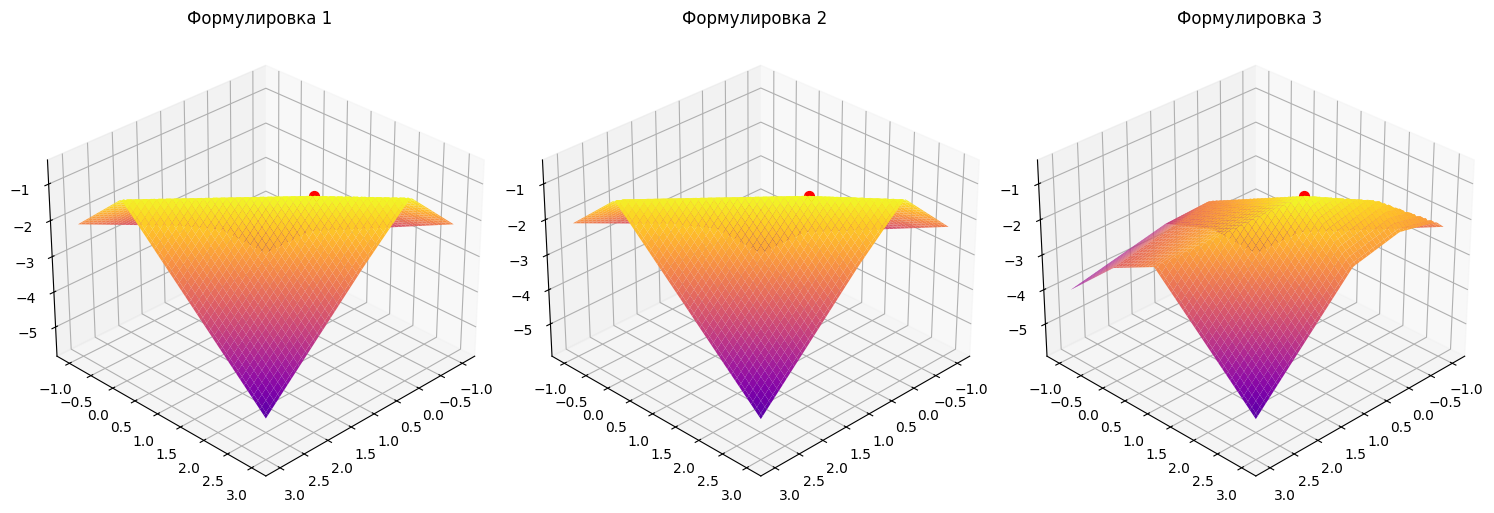
\includegraphics[width = \textwidth]{tol}
            \caption{Расположение максимума распознающего функционала}
    \label{figure:tol}
        \end{center}
    \end{figure}

    \subsection{Достижение разрешимости за счёт коррекции левой части (A-коррекция)}

    Для обеспечения разрешимости системы с использованием \( A \)-коррекции в формулировке (\ref{eq:problem_1}) выполним следующие шаги:
    
    \begin{enumerate}
      \item \textbf{Определение исходных параметров.} Для текущих значений системы значение толерантности вычисляется как 
      \[
      T = \text{Tol}(\tau, \mathbf{A}, \mathbf{b}) = -0.7 \Rightarrow |T| = 0.7.
      \]
      Максимум распознающего функционала достигается в точке 
      \[
      \tau = \text{Arg} \max_{x \in \mathbb{R}^n} \text{Tol}(x, \mathbf{A}, \mathbf{b}) = (1, 2)^T,
      \]
      откуда \( |\tau_1| = 1 \) и \( |\tau_2| = 2 \).
      
      \item \textbf{Вычисление радиуса матрицы.} Радиус элементов матрицы \(\mathbf{A}\) определяется как 
      \[
      \text{rad} A = \begin{pmatrix}
          0.3 & 0.3 \\
          0.3 & 0.3 \\
          0.3 & 0.3 \\
          0.3 & 0.3
      \end{pmatrix}.
      \]
    
      \item \textbf{Нахождение интервала корректировки.} Составим и решим систему неравенств для интервала допустимых значений \( e \), учитывая ограничение на радиус коррекции:
      \[
      \begin{cases}
        0 \leqslant e \leqslant 0.3, \\
        e + 2e = K \geqslant |T| = 0.7.
      \end{cases}
      \]
      Решая эту систему, получаем:
      \[
      0.2(3) \leqslant e \leqslant 0.3.
      \]
    
      \item \textbf{Выбор оптимального значения.} Для дальнейших расчётов выберем среднее значение в найденном интервале:
      \[
      e_{\text{mid}} = \frac{0.2(3) + 0.3}{2} = 0.2(6).
      \]
    
      \item \textbf{Построение скорректированной системы.} С учётом выбранного значения \( e_{\text{mid}} \), интервальная система принимает следующий вид:
      \[
      \mathbf{A} = \begin{pmatrix}
          [0.917, 0.983] & [0.967, 1.033] \\
          [1.017, 1.083] & [0.967, 1.033] \\
          [1.067, 1.133] & [0.967, 1.033] \\
          [-0.033, 0.033] & [0.967, 1.033]
      \end{pmatrix}, \quad
      \mathbf{b} = \begin{pmatrix}
          [2.75, 3.15] \\
          [2.85, 3.25] \\
          [2.90, 3.3] \\
          [1.8, 2.2]
      \end{pmatrix}.
      \]
    \end{enumerate}

  Максимум со значением \( T = 0.1 \) расположен в точке
  \( \tau = (1, 2)^T \).

  \begin{figure}[H]
		\begin{center}
			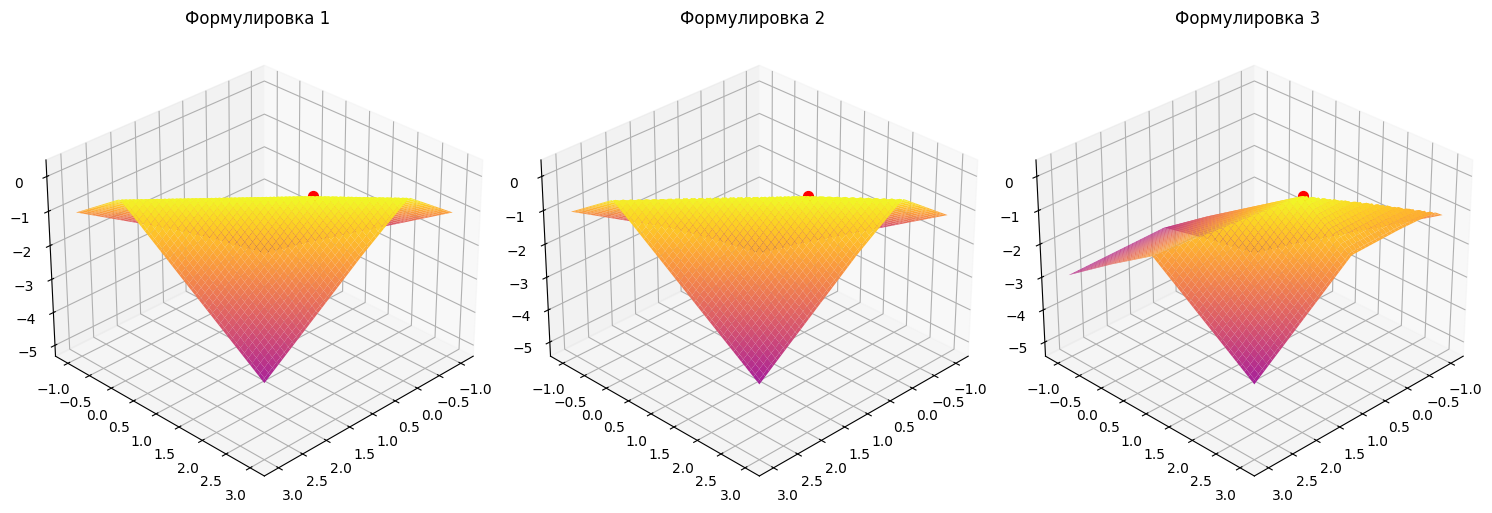
\includegraphics[width = \textwidth]{tol_a_corrected}
			\caption{Поверхности распознающих функционалов после
        \( A \)-корректировки}
      \label{figure:tol_a_corrected}
		\end{center}
	\end{figure}

  \begin{figure}[H]
		\begin{center}
			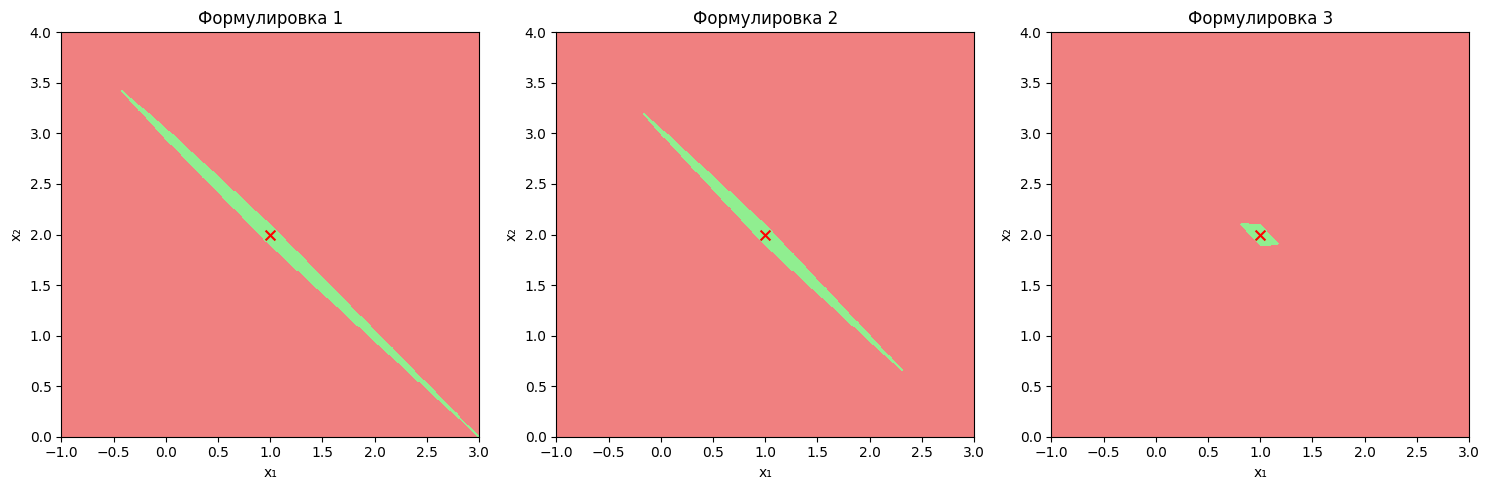
\includegraphics[width = \textwidth]{tol_functional_a_corrected}
			\caption{Допусковое множество решений после \( A \)-корректировки}
      \label{figure:tol_functional_a_corrected}
		\end{center}
	\end{figure}

\subsection{Достижение разрешимости за счёт коррекции правой части (b-коррекция)}

Для формирования интервальной матрицы использовался коэффициент \( K = 1 \) для всех рассматриваемых ИСЛАУ. Например, задача \ref{eq:problem_3} принимает следующий вид:

\[
\mathbf{A} = \begin{pmatrix}
  [0.65, 1.25] & [0.7, 1.3] \\
  [0.75, 1.35] & [0.7, 1.3] \\
  [0.8, 1.4] & [0.7, 1.3] \\
  [-0.3, 0.3] & [0.7, 1.3]
\end{pmatrix}, \quad
\mathbf{b} = \begin{pmatrix}
  [1.75, 4.15] \\
  [1.85, 4.25] \\
  [1.9, 4.3] \\
  [0.8, 3.2]
\end{pmatrix}.
\]

\begin{figure}[H]
  \centering
  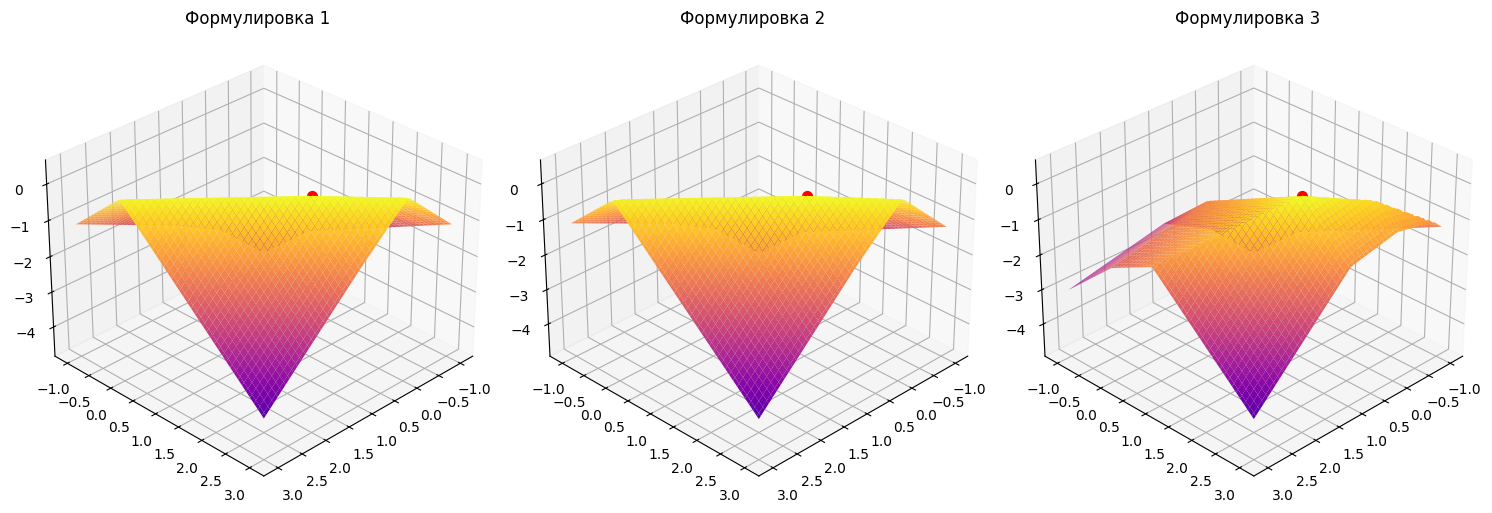
\includegraphics[width=\textwidth]{tol_b_corrected}
  \caption{Поверхности распознающих функционалов после \( b \)-коррекции}
  \label{figure:tol_b_corrected}
\end{figure}

\begin{figure}[H]
  \centering
  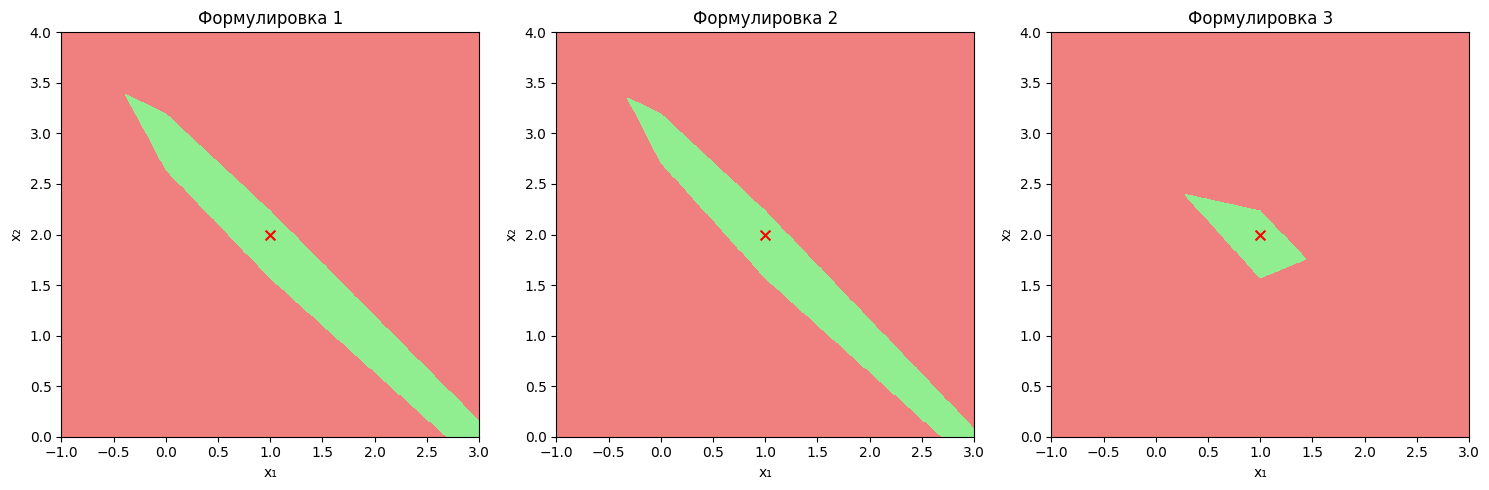
\includegraphics[width=\textwidth]{tol_functional_b_corrected}
  \caption{Допусковое множество решений после \( b \)-коррекции}
  \label{figure:tol_functional_b_corrected}
\end{figure}

Минимальное значение коэффициента \( K \), равное \( 0.7 \), в предельном случае неотрицательной области сходится к точке \( \tau = (1, 2)^T \).



\subsection{Достижение разрешимости за счёт Ab-коррекции}

Процесс включал два этапа: сначала выполнялось сужение левой части (\( A \)-коррекция), а затем — расширение правой части (\( b \)-коррекция) с коэффициентом \( K = 1 \).

\begin{figure}[H]
    \begin{center}
        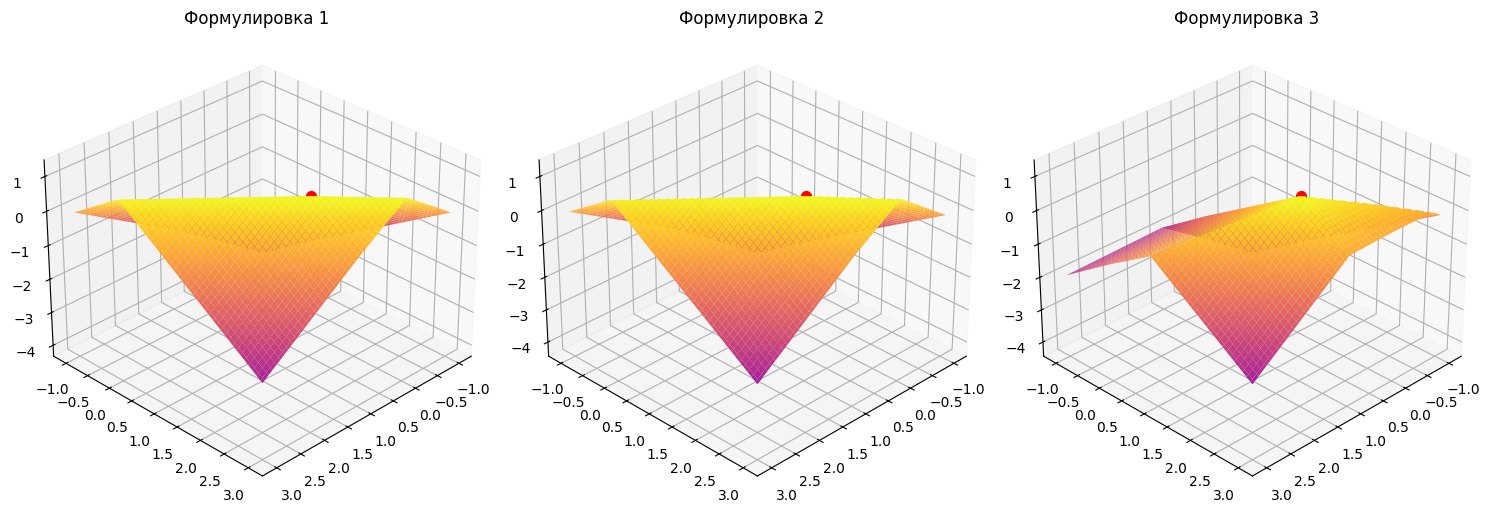
\includegraphics[width = \textwidth]{tol_ab_corrected}
        \caption{Поверхности распознающих функционалов после
    \( Ab \)-корректировки}
  \label{figure:tol_ab_corrected}
    \end{center}
\end{figure}

\begin{figure}[H]
    \begin{center}
        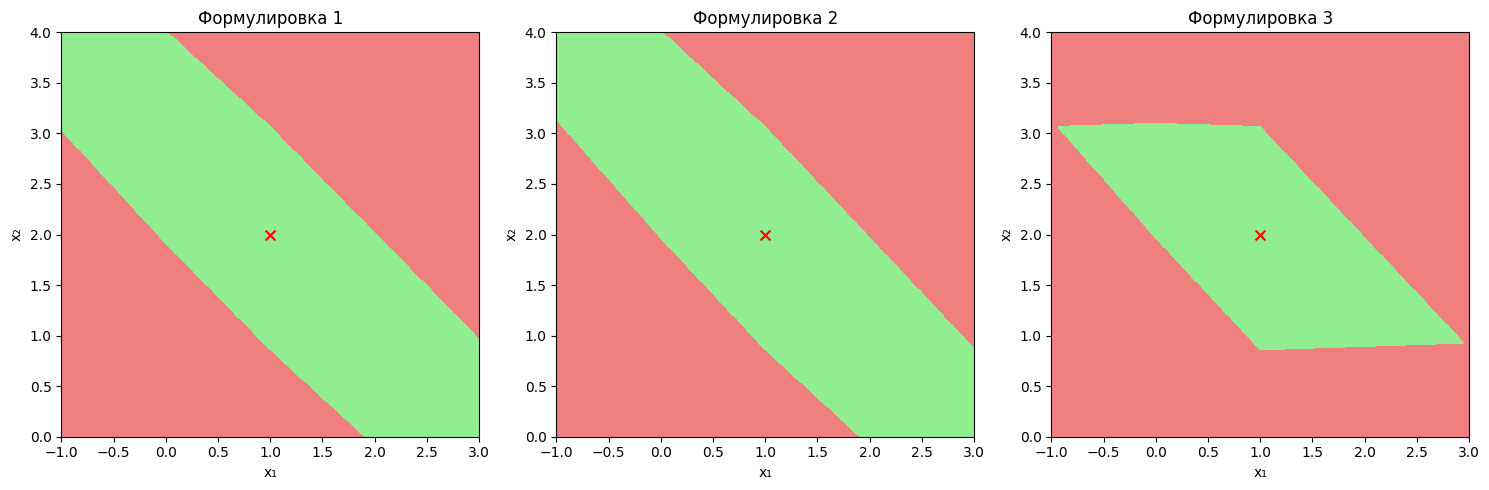
\includegraphics[width = \textwidth]{tol_functional_ab_corrected}
        \caption{Допусковое множество решений после \( Ab \)-корректировки}
  \label{figure:tol_functional_ab_corrected}
    \end{center}
\end{figure}


\section{Выводы}

\begin{itemize}
  \item Проведённый анализ показал, что для исходных ИСЛАУ допусковое множество решений отсутствует, так как максимальное значение распознающего функционала \( T = -0.7 \) оказалось отрицательным. Это свидетельствует о несовместимости системы в заданных интервалах.
  \item Для устранения несовместимости были использованы методы коррекции правой части (\( b \)-коррекция) и матрицы коэффициентов (\( A \)-коррекция). В результате применения \( b \)-коррекции с коэффициентом \( K = 1 \) удалось достичь положительного значения распознающего функционала \( T = 0.3 \), что подтверждает наличие допускового множества решений для скорректированной системы.
  \item Метод \( A \)-коррекции также обеспечил разрешимость системы. Корректировка матрицы коэффициентов привела к положительному значению распознающего функционала, что позволило определить допусковое множество решений и подтвердить эффективность данного подхода.
  \item Анализ графиков допусковых множеств и распознающего функционала показал, что после коррекции изменился профиль поверхности \( \text{Tol}(x) \). Это свидетельствует о влиянии коррекции на свойства системы. Кроме того, смещение максимума распознающего функционала указывает на улучшение совместимости системы.
\end{itemize}
\end{document}
